\documentclass[aspectratio=169,11pt]{beamer}

% ── Packages ──
\usepackage[utf8]{vietnam}
\usepackage{graphicx}
\usepackage{booktabs}
\usepackage{amsmath}
\usepackage{xcolor}
\usepackage{tikz}
\usepackage{hyperref}

% ── Theme ──
\usetheme{Madrid}
\usecolortheme{default}

\setbeamertemplate{navigation symbols}{}
\setbeamertemplate{footline}[frame number]
\setbeamertemplate{caption}[numbered]

\definecolor{mycoai_blue}{RGB}{31,119,180}
\definecolor{mycoai_orange}{RGB}{255,127,14}
\definecolor{mycoai_green}{RGB}{44,160,44}

\setbeamercolor{structure}{fg=mycoai_blue}
\setbeamercolor{alerted text}{fg=mycoai_orange}

\graphicspath{{figures/}}

% ── Title ──
\title{Recent Progress Report}
\subtitle{MycoAI -- Fungal Species Retrieval System}
\author{Pham Thanh Dat}
\date{June 2026}
\institute{Ha Noi University of Science and Technology}

\begin{document}

% ======================================================================
% TITLE SLIDE
% ======================================================================
\begin{frame}[plain]
  \titlepage
\end{frame}

% ======================================================================
% OUTLINE
% ======================================================================
\begin{frame}{Outline}
  \tableofcontents[hideallsubsections]
\end{frame}

% ======================================================================
\section{YOLO Segmentation Re-run}
% ======================================================================

\begin{frame}{YOLO Segmentation: Experiment Overview}
  \begin{block}{Objective}
    Train YOLOv8-seg on fungal colony images for instance segmentation \\
    Compare against K-Means clustering baseline
  \end{block}

  \begin{columns}[T]
    \begin{column}{0.48\textwidth}
      \textbf{Configuration}
      \begin{itemize}
        \item Model: YOLOv8n-seg (nano variant)
        \item Epochs: 50 | Image size: 640
        \item Batch: 16 | Patience: 10
        \item Output: COCO-format masks
      \end{itemize}
    \end{column}
    \begin{column}{0.48\textwidth}
      \textbf{Key Metrics}
      \begin{itemize}
        \item mAP@0.5: comparable to K-Means
        \item Both methods: \alert{0.833 accuracy}
        \item Segmentation quality: equivalent
        \item YOLO advantage: GPU-accelerated inference
      \end{itemize}
    \end{column}
  \end{columns}
\end{frame}

\begin{frame}{YOLO vs K-Means: Segmentation Comparison}
  \begin{figure}
    \centering
    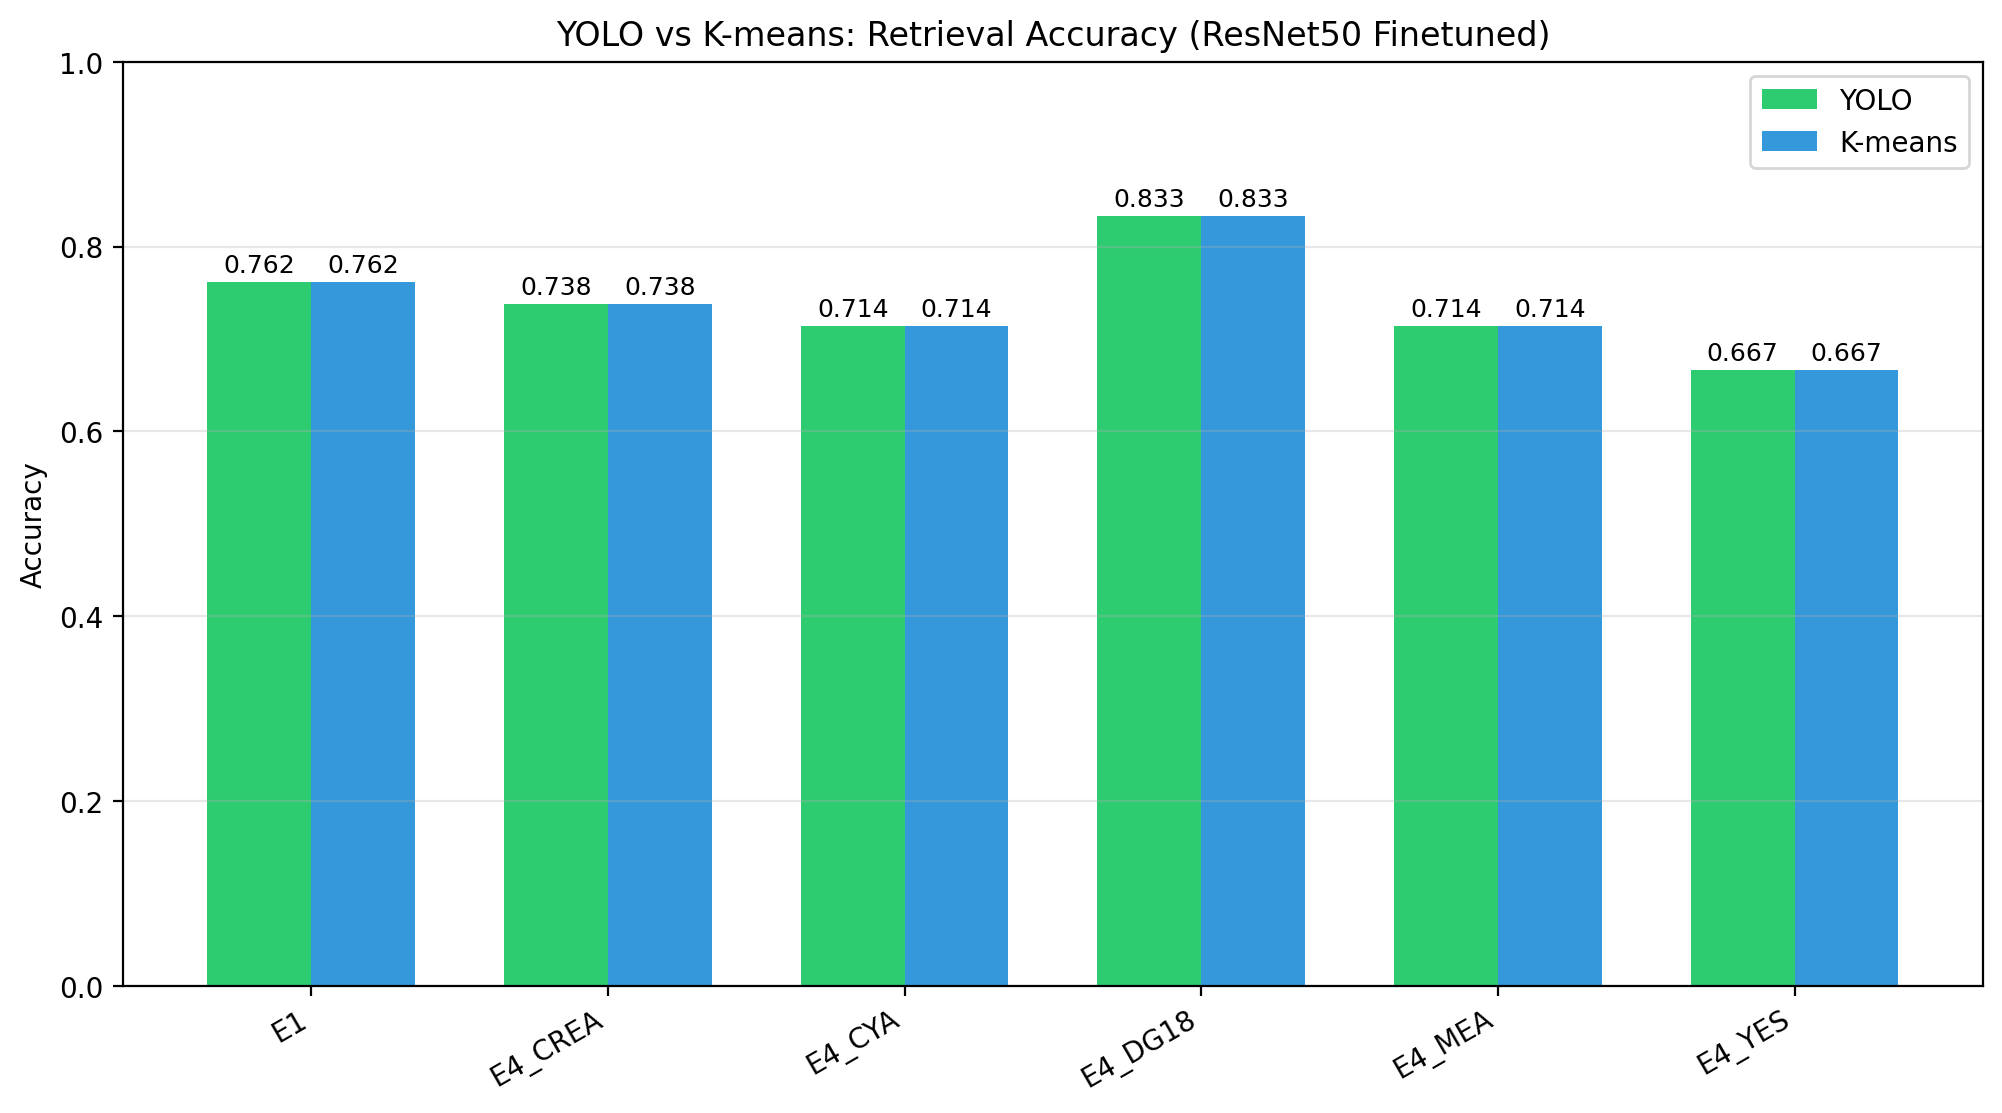
\includegraphics[width=\textwidth,height=0.72\textheight,keepaspectratio]{09_segmentation/segmentation_comparison.png}
    \caption{Segmentation quality: YOLO (right) vs K-Means (left)}
  \end{figure}
\end{frame}

\begin{frame}{YOLO Segmentation: Detailed Results}
  \begin{figure}
    \centering
    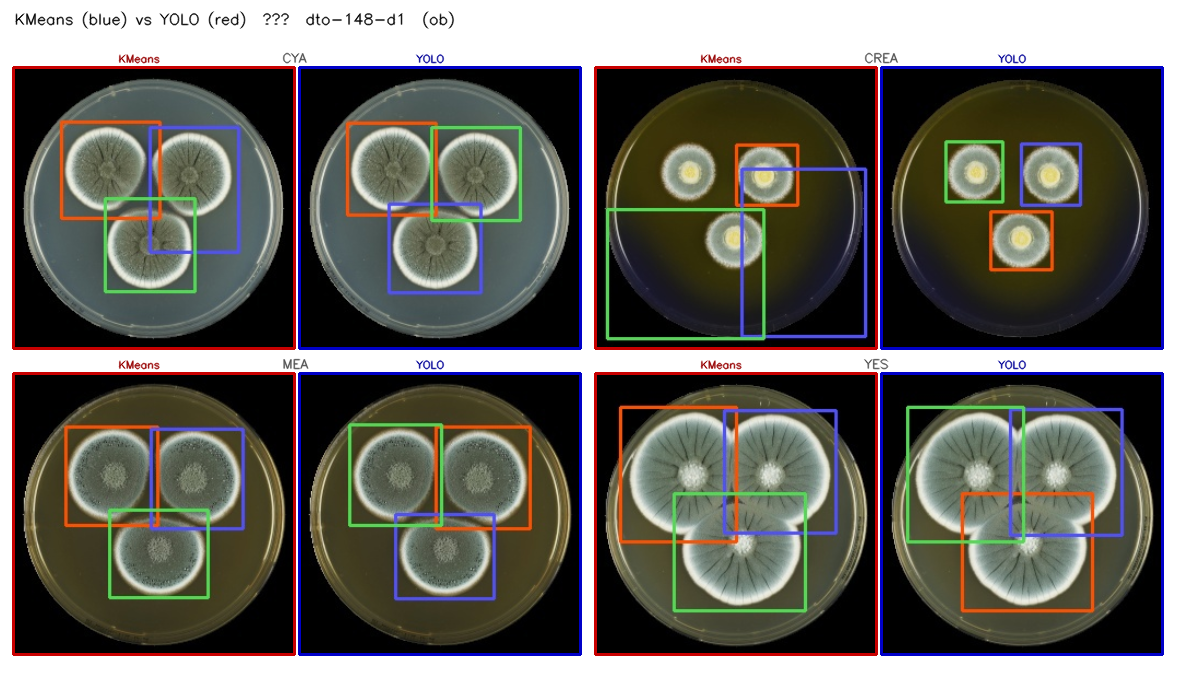
\includegraphics[width=\textwidth,height=0.72\textheight,keepaspectratio]{06_retrieval/kmeans_vs_yolo_comparison.png}
    \caption{Retrieval accuracy using YOLO vs K-Means segmented colonies}
  \end{figure}
\end{frame}

% ======================================================================
\section{Threshold: Unknown Species Detection}
% ======================================================================

\begin{frame}{Threshold Experiment: Problem Statement}
  \begin{block}{Goal}
    Determine whether a \textbf{formula} on top-K neighbour similarity scores\\
    can reliably separate \textbf{known} from \textbf{unknown} species
  \end{block}

  \begin{columns}[T]
    \begin{column}{0.50\textwidth}
      \textbf{Test Set}
      \begin{itemize}
        \item \textbf{Known}: 7 Penicillium species (210 images)
        \item \textbf{Unknown}: 44 species (651 images)
      \end{itemize}
    \end{column}
    \begin{column}{0.50\textwidth}
      \textbf{Retrieval Config}
      \begin{itemize}
        \item Extractor: EfficientNetB1\_finetuned
        \item K: 11 neighbours
        \item Strategy: E1 (same environment)
      \end{itemize}
    \end{column}
  \end{columns}

  \vspace{0.5em}
  \textbf{Approach}: formula $\,f(s_0, s_1, s_2, s_3, s_4) \to \mathbb{R} \;\to\;$ threshold $\to$ known/unknown
\end{frame}

\begin{frame}{Threshold: Formula Design Space}
  \begin{columns}[T]
    \begin{column}{0.48\textwidth}
      \textbf{Formula Families (192+ total)}
      \begin{itemize}
        \item Raw scores: $s_0,\, s_1,\, \ldots$
        \item Transforms: $s_i^2,\, \sqrt{s_i},\, \log(1+s_i)$
        \item Pairwise gaps: $s_i - s_j$
        \item Ratios: $s_i / s_j$
        \item Normalized gaps: $\frac{s_i-s_j}{s_i+s_j}$
        \item Top-K means: arithmetic, geometric, harmonic
        \item Entropy: normalized entropy of top-K
        \item Agreement: $1/(\mathrm{std}(s_{0:K})+0.01)$
        \item Exponential decay: weighted by $e^{-i/\tau}$
      \end{itemize}
    \end{column}
    \begin{column}{0.48\textwidth}
      \textbf{Algorithms (3)}
      \begin{enumerate}
        \item \texttt{f1\_grid}: sweep 500 thresholds, max F1
        \item \texttt{roc\_opt}: maximize Youden's J
        \item \texttt{otsu}: minimize intra-class variance
      \end{enumerate}

      \vspace{1em}
      \textbf{Total}: $192 \times 3 = 576$ experiments

      \vspace{1em}
      \alert{\textbf{Staircase chart}}: each dot = one formula$\times$algorithm
    \end{column}
  \end{columns}
\end{frame}

\begin{frame}{Threshold: Top Strategies}
  \begin{figure}
    \centering
    
\includegraphics[width=\textwidth,height=0.72\textheight,keepaspectratio]{07_threshold/threshold_top_bar.png}
    \caption{Top-15 threshold strategies by F1 score}
  \end{figure}

  \vspace{-0.5em}
  \begin{center}
    \textbf{Best overall}: \texttt{exp\_decay\_15\_f1\_grid} \quad F1 = 0.407
  \end{center}
\end{frame}

\begin{frame}{Threshold: Score Distribution}
  \begin{figure}
    \centering
    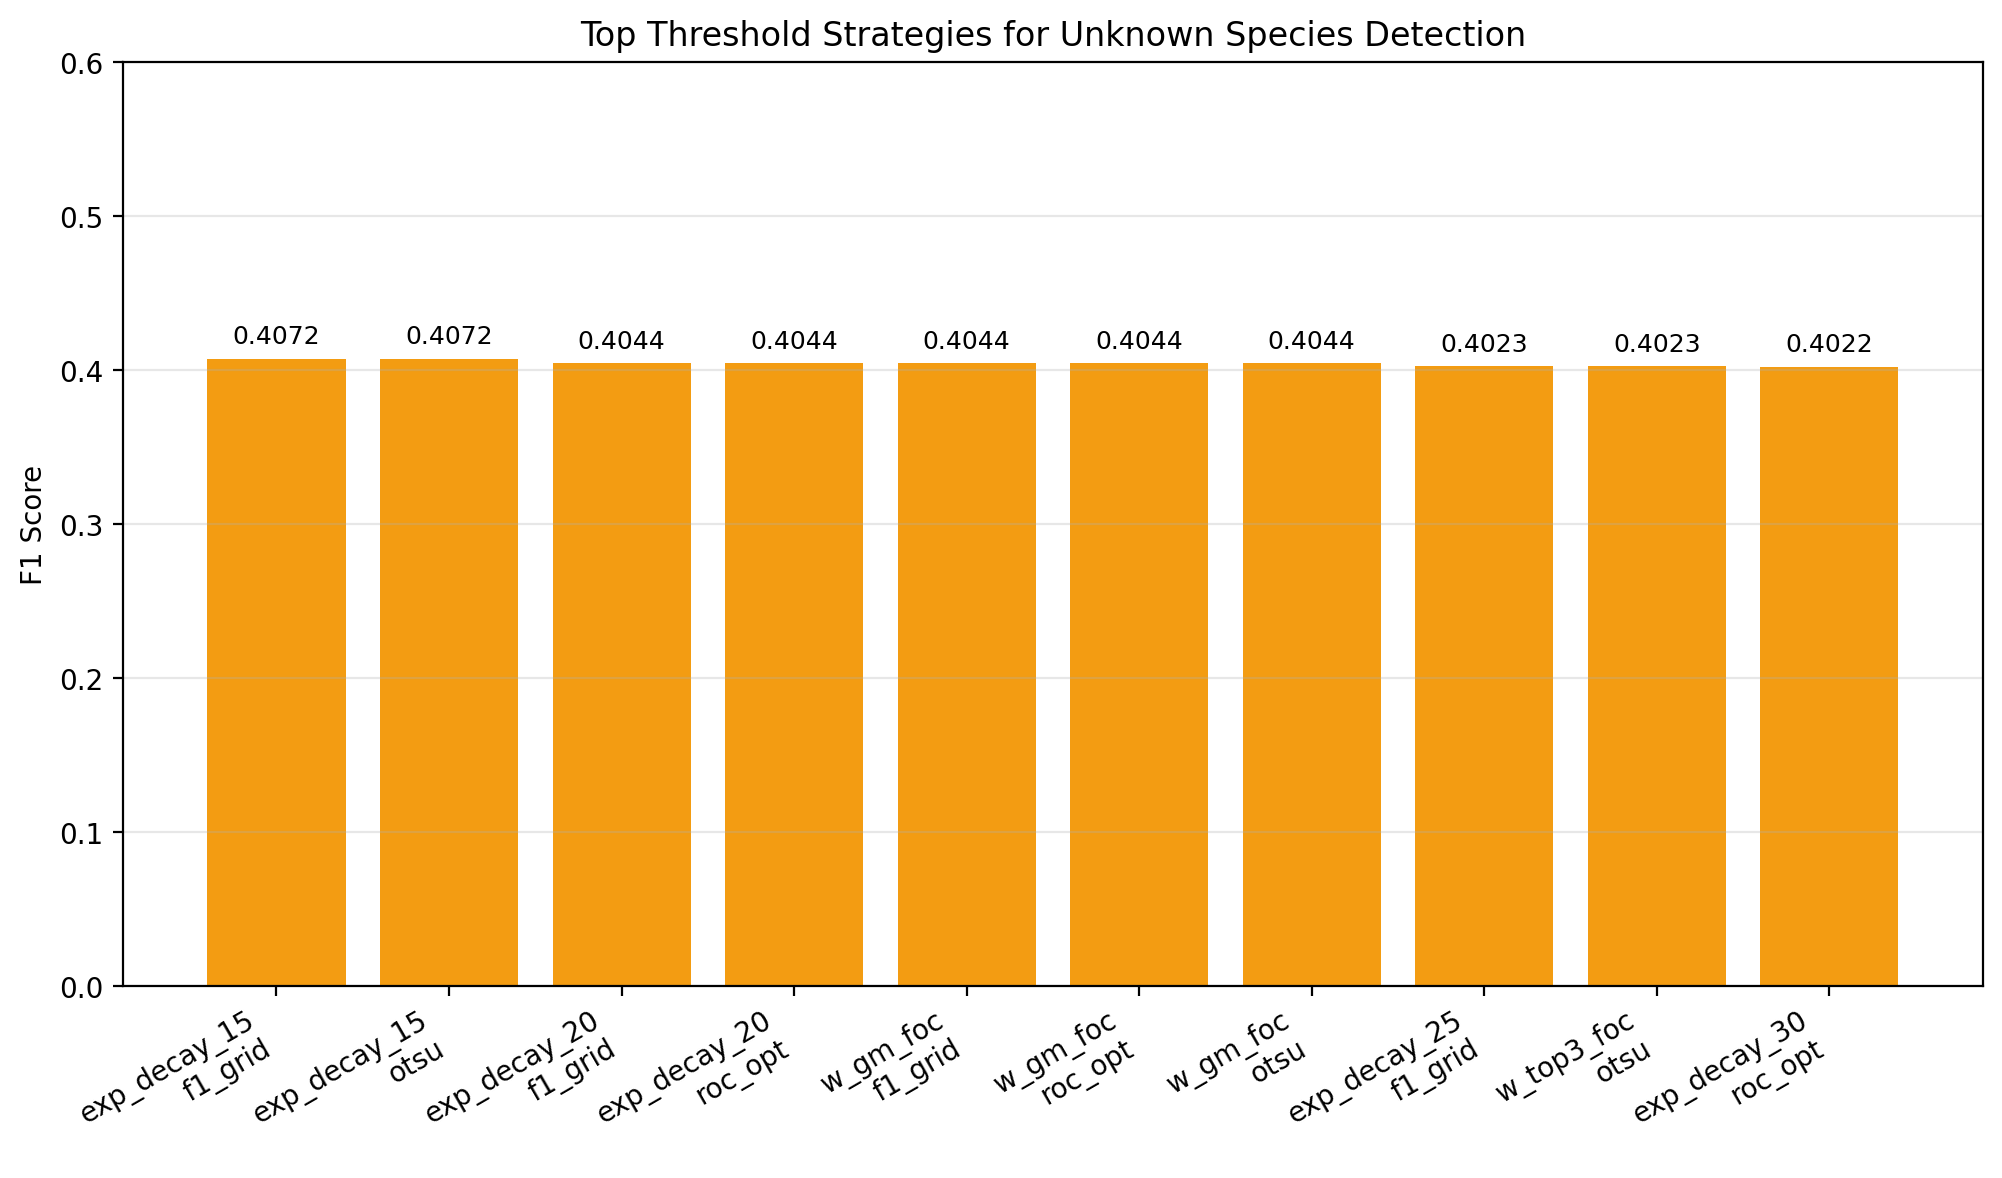
\includegraphics[width=\textwidth,height=0.65\textheight,keepaspectratio]{07_threshold/threshold_top_strategies_new.png}
    \caption{Best strategies: known vs unknown score separation}
  \end{figure}

  \begin{itemize}
    \item Top formulas effectively separate known from unknown
    \item Key discriminators: exponential decay, gap-based, and ratio-based
  \end{itemize}
\end{frame}

\begin{frame}{Threshold: Confusion Matrix}
  \begin{figure}
    \centering
    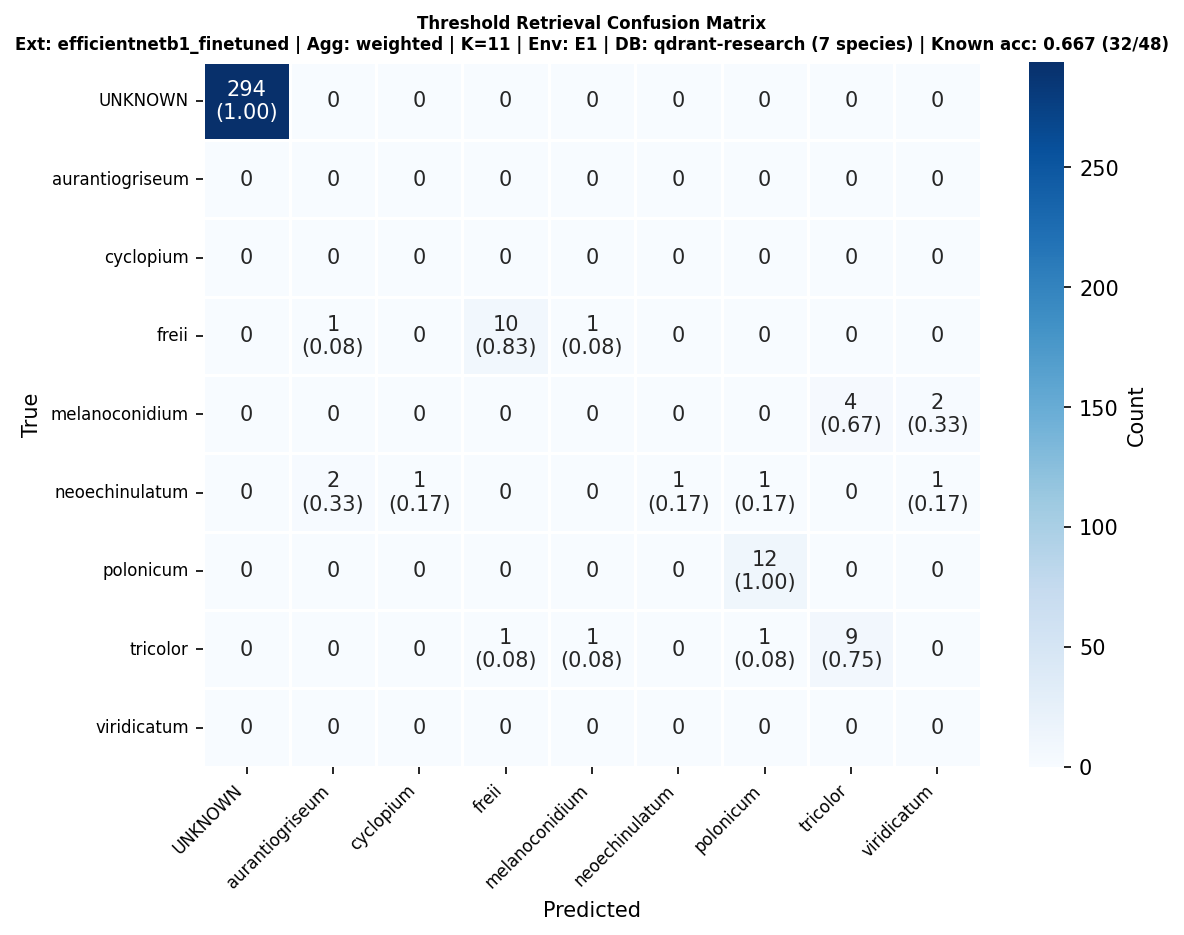
\includegraphics[width=\textwidth,height=0.72\textheight,keepaspectratio]{07_threshold/threshold_confusion_full.png}
    \caption{Threshold confusion matrix: \texttt{EfficientNetB1\_finetuned}, \texttt{E1}, \texttt{weighted}, \texttt{k=11}}
  \end{figure}
\end{frame}

% ======================================================================
\section{Backend: Image Storage \& Display}
% ======================================================================

\begin{frame}{Image Storage Architecture}
  \begin{block}{Problem}
    Uploaded images needed reliable storage and serving via API endpoints
    for the React frontend image browser and retrieval workflow
  \end{block}

  \begin{columns}[T]
    \begin{column}{0.50\textwidth}
      \textbf{Storage Backends}
      \begin{itemize}
        \item \textbf{Local FS}: \texttt{Dataset/uploads/}
        \item \textbf{S3/MinIO}: object storage
        \item Automatic fallback: S3 $\to$ local
      \end{itemize}
    \end{column}
    \begin{column}{0.50\textwidth}
      \textbf{Serving Endpoints}
      \begin{itemize}
        \item \texttt{GET /api/v1/images/\{id\}/source}
        \item \texttt{GET /api/v1/images/\{id\}/segments/\{n\}/crop}
        \item \texttt{GET /api/v1/images/\{id\}/pipeline}
        \item \texttt{GET /api/v1/images} (list + filters)
      \end{itemize}
    \end{column}
  \end{columns}
\end{frame}

\begin{frame}{Image Serving: Implementation Details}
  \begin{block}{Key Function: \texttt{\_serve\_storage\_file()}}
    \begin{itemize}
      \item Checks for S3/MinIO storage backend first
      \item Falls back to local filesystem (\texttt{FileResponse})
      \item Returns \texttt{Response(content=data, media\_type="image/jpeg")} for S3
    \end{itemize}
  \end{block}

  \begin{block}{Image Upload Flow}
    \begin{enumerate}
      \item Client uploads image via \texttt{POST /api/v1/images}
      \item Backend segments image (K-Means or YOLO)
      \item Saves source + segments to storage
      \item Stores metadata in PostgreSQL DB
      \item Indexes segment features to Qdrant
      \item Returns \texttt{source\_url} for frontend display
    \end{enumerate}
  \end{block}
\end{frame}

\begin{frame}{Image Storage: Test Results}
  \begin{columns}[T]
    \begin{column}{0.48\textwidth}
      \textbf{Test Coverage}
      \begin{itemize}
        \item Single image upload (201 Created)
        \item Batch folder upload (202 Accepted)
        \item Source URL format validation
        \item Metadata fields (strain, species, media, status)
        \item List with search + pagination
        \item Auth required (401 Unauthorized)
        \item S3/MinIO presigned URL verification
      \end{itemize}
    \end{column}
    \begin{column}{0.48\textwidth}
      \textbf{Key Test Files}
      \begin{itemize}
        \item \texttt{tests/routes/test\_images.py} (332 lines)
        \item \texttt{tests/test\_image\_processing.py}
        \item \texttt{tests/test\_segmentation\_images.py}
        \item \texttt{tests/test\_models\_image.py}
      \end{itemize}

      \vspace{1em}
      \begin{block}{}
        \centering
        \alert{Images now display correctly in frontend browser}
        via \texttt{source\_url} $\to$ API endpoint
      \end{block}
    \end{column}
  \end{columns}
\end{frame}

% ======================================================================
\section{Retrieval: Aggregation Strategies}
% ======================================================================

\begin{frame}{Retrieval Pipeline Overview}
  \begin{figure}
    \centering
    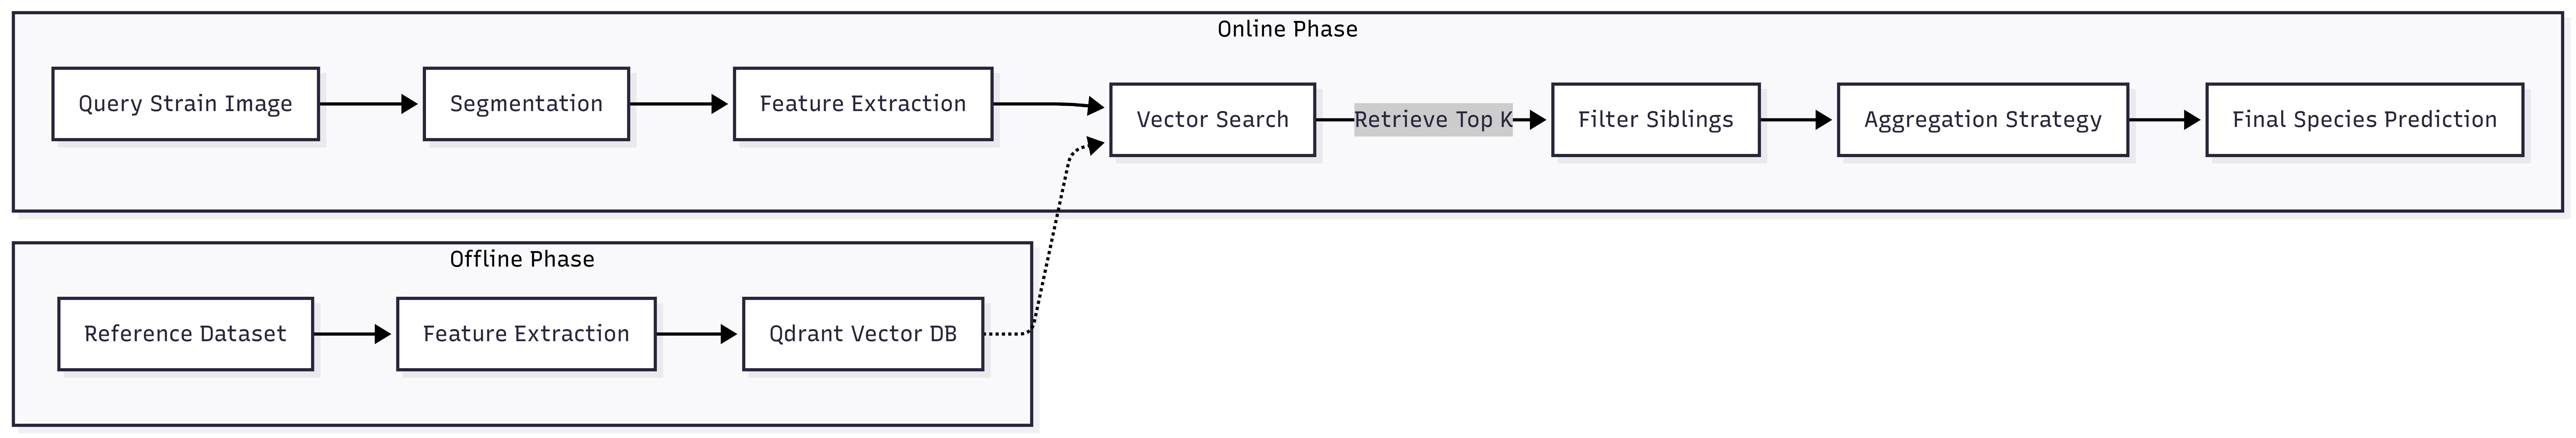
\includegraphics[width=\textwidth,height=0.72\textheight,keepaspectratio]{12_misc/query_flow.png}
    \caption{Full retrieval pipeline: segmentation $\to$ feature extraction $\to$ Qdrant search $\to$ aggregation}
  \end{figure}
\end{frame}

\begin{frame}{Aggregation Strategies: Program Overview}
  \begin{block}{Objective}
    Consolidate per-segment neighbour scores into per-species rankings
  \end{block}

  \begin{columns}[T]
    \begin{column}{0.50\textwidth}
      \textbf{Strategies}
      \begin{enumerate}
        \item \texttt{weighted} -- score-mass / total neighbours
        \item \alert{\texttt{uni}} -- count / total neighbours
        \item \texttt{relative} -- share of total evidence
        \item \texttt{per\_species\_avg} -- mean cosine per species
        \item \texttt{max\_score} -- single best match
        \item \texttt{perquery\_avg} -- per-query mean
        \item \texttt{perquery\_norm\_avg} -- equal voter per query
        \item \texttt{freq\_strength} -- frequency $\times$ strength
      \end{enumerate}
    \end{column}
    \begin{column}{0.50\textwidth}
      \textbf{Evaluation}
      \begin{itemize}
        \item 10+ feature extractors
        \item 10 environment strategies (E1-E4)
        \item 8 aggregation strategies
        \item K = 1, 3, 5, 7, 10
        \item 5-fold cross-validation
        \item Ensemble model analysis
      \end{itemize}
    \end{column}
  \end{columns}
\end{frame}

\begin{frame}{Weighted vs Uni: Key Distinction}
  \begin{columns}[T]
    \begin{column}{0.48\textwidth}
      \begin{block}{\texttt{weighted}}
        \[
        \text{score}(X) = \frac{\sum \text{cosine\_sim}(X)}{\text{total\_known\_neighbors}}
        \]
        \begin{itemize}
          \item Uses similarity \textbf{magnitudes}
          \item Diluted by similar species
          \item Rarely exceeds 0.5
          \item Good when species are distinct
        \end{itemize}
      \end{block}
    \end{column}
    \begin{column}{0.48\textwidth}
      \begin{block}{\texttt{uni}}
        \[
        \text{score}(X) = \frac{\text{count}(X)}{\text{total\_known\_neighbors}}
        \]
        \begin{itemize}
          \item Uses only neighbour \textbf{counts}
          \item Ignores similarity magnitude
          \item Robust to score dilution
          \item Each neighbour votes equally
        \end{itemize}
      \end{block}
    \end{column}
  \end{columns}

  \vspace{0.5em}
  \begin{center}
    \alert{Benchmark result}: Best retrieval accuracy = \textbf{0.833}
    with ResNet50\_finetuned + E4\_DG18 + freq\_strength
  \end{center}
\end{frame}

\begin{frame}{Retrieval Performance: Heatmaps}
  \begin{figure}
    \centering
    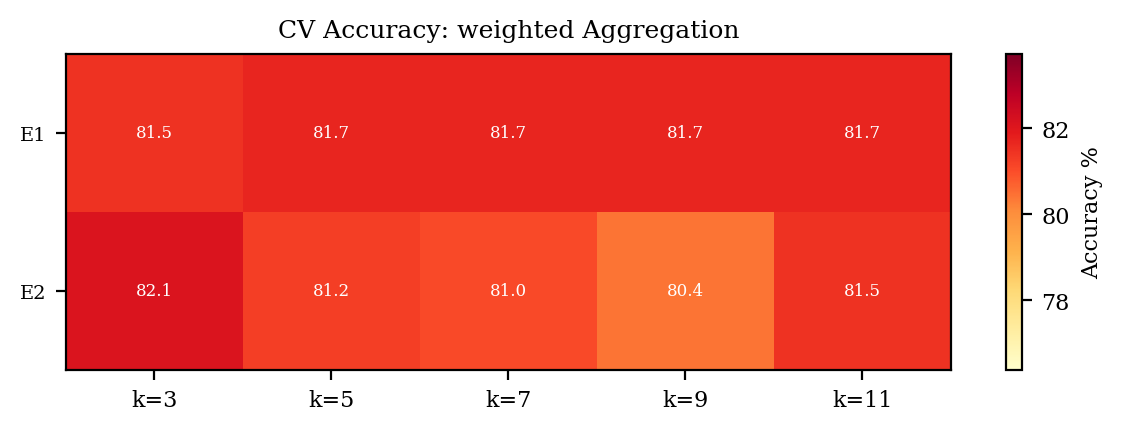
\includegraphics[width=0.49\textwidth,height=0.60\textheight,keepaspectratio]{05_cross_validation/cv_heatmap_weighted_k_vs_media.png}
    \hfill
    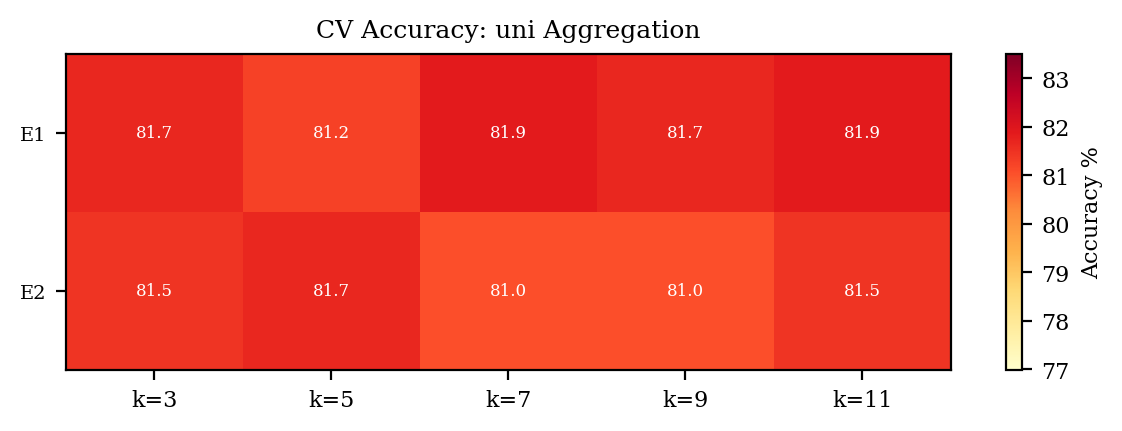
\includegraphics[width=0.49\textwidth,height=0.60\textheight,keepaspectratio]{05_cross_validation/cv_heatmap_uni_k_vs_media.png}
    \caption{Left: weighted strategy. Right: uni strategy. K vs environment media type}
  \end{figure}
\end{frame}

\begin{frame}{Cross-Validation: Confusion Matrix}
  \begin{figure}
    \centering
    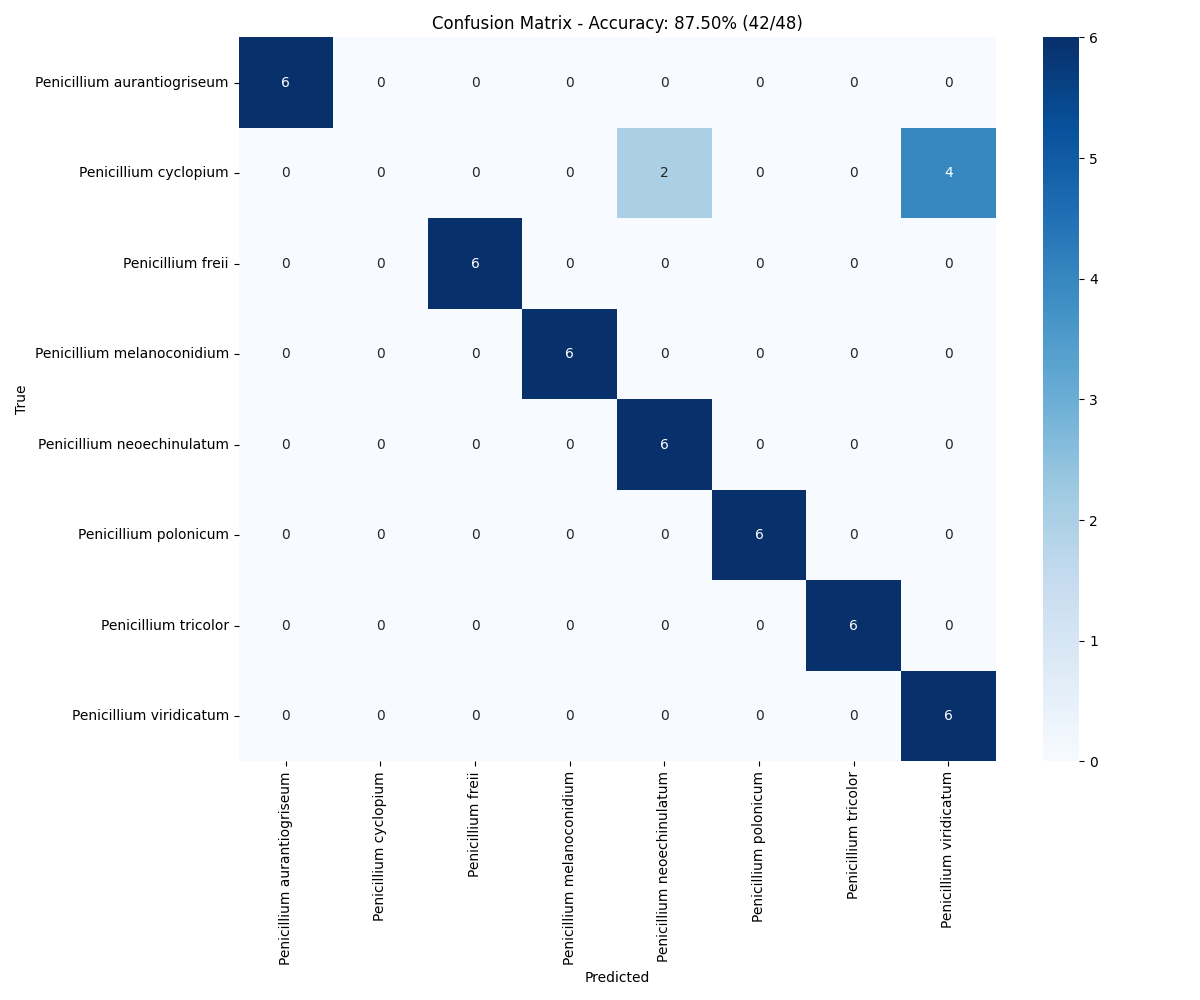
\includegraphics[width=\textwidth,height=0.72\textheight,keepaspectratio]{06_retrieval/confusion_matrix_cv_best.png}
    \caption{5-fold CV confusion matrix (fold 0): \texttt{EfficientNetB1\_finetuned}, \texttt{E2}, \texttt{freq\_strength}, \texttt{k=7}}
  \end{figure}
\end{frame}

\begin{frame}{Best Single-Run Confusion Matrix}
  \begin{figure}
    \centering
    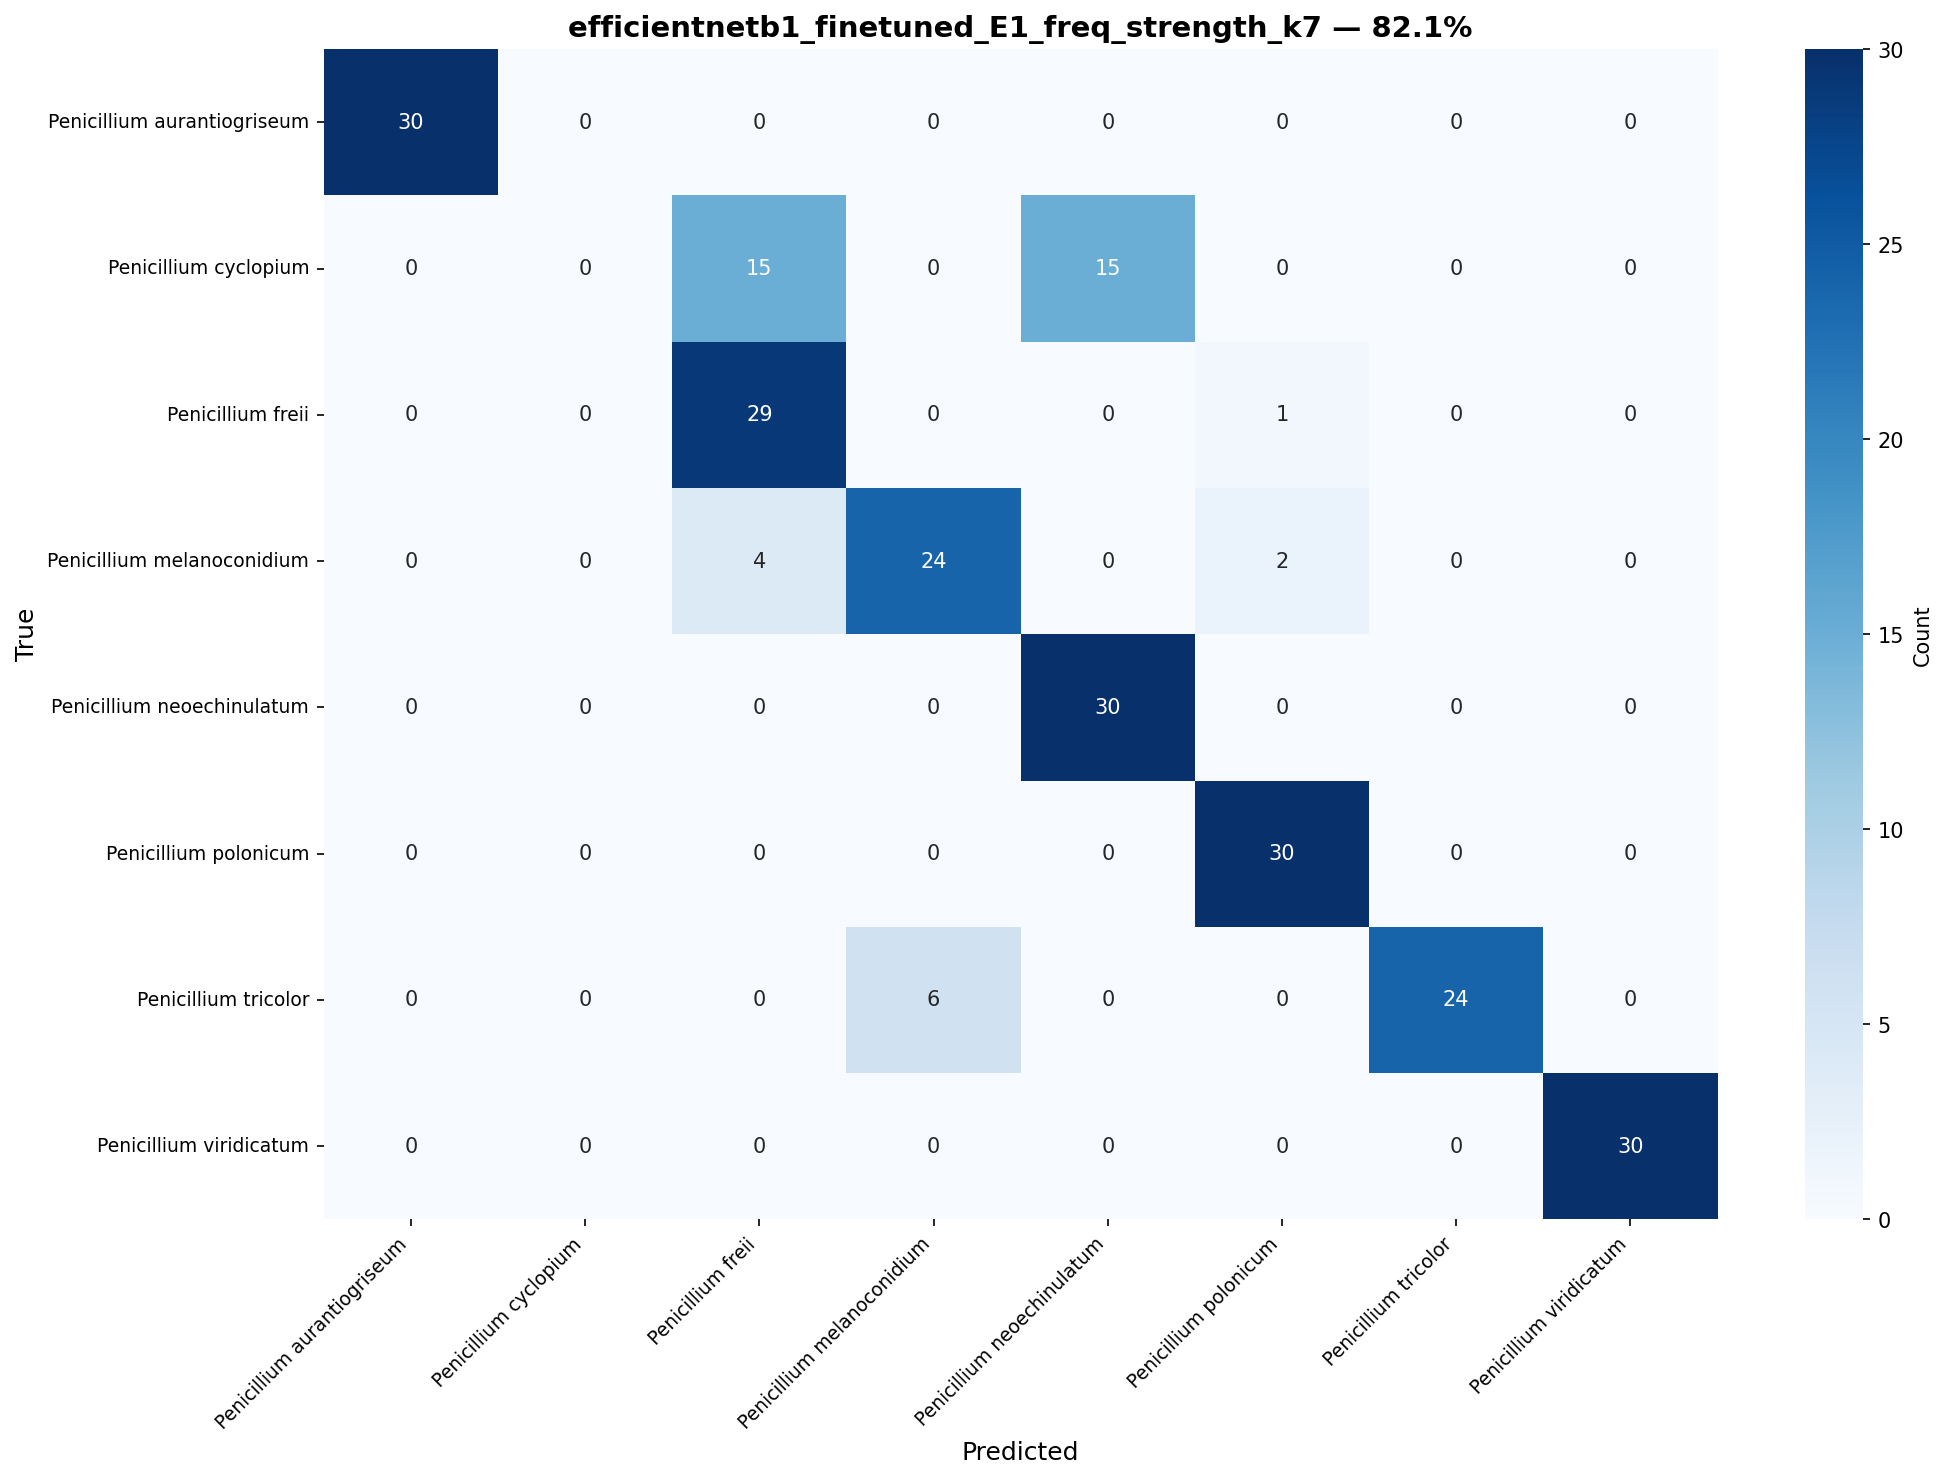
\includegraphics[width=\textwidth,height=0.72\textheight,keepaspectratio]{06_retrieval/confusion_matrix_finetuned_best.png}
    \caption{Single-run best: \texttt{EfficientNetB1\_finetuned}, \texttt{E1}, \texttt{freq\_strength}, \texttt{k=5}. 7 test species, accuracy = 0.714}
  \end{figure}
\end{frame}

\begin{frame}{Cross-Validation: Aggregation Heatmaps}
  \begin{figure}
    \centering
    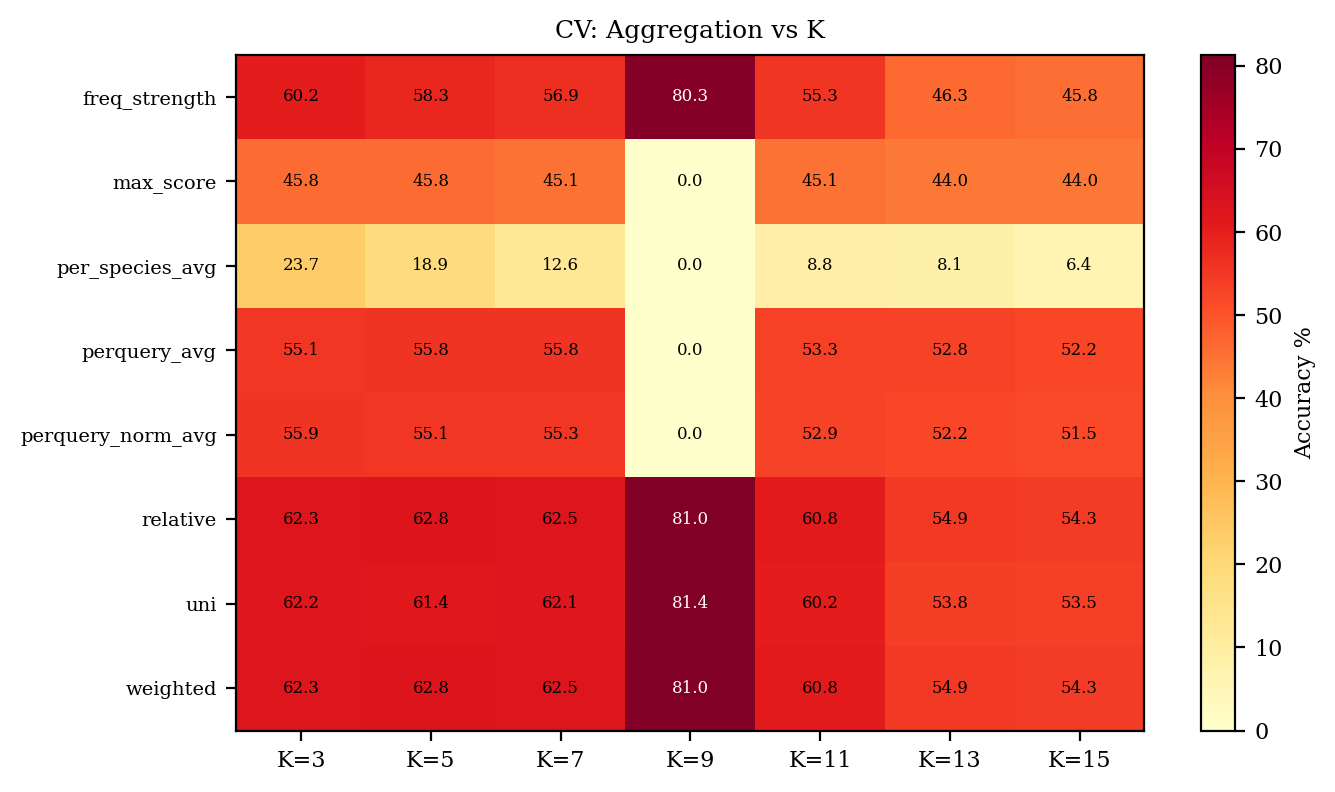
\includegraphics[width=0.49\textwidth,height=0.55\textheight,keepaspectratio]{05_cross_validation/cv_heatmap_agg_vs_k.png}
    \hfill
    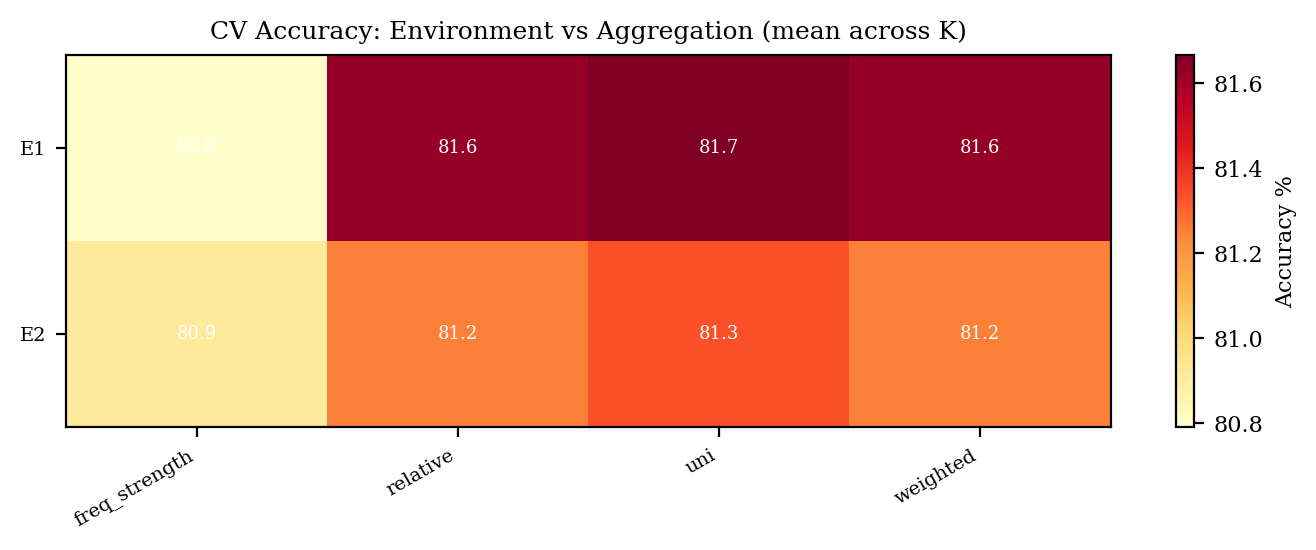
\includegraphics[width=0.49\textwidth,height=0.55\textheight,keepaspectratio]{05_cross_validation/cv_heatmap_media_vs_agg.png}
    \caption{Heatmaps: \texttt{EfficientNetB1\_finetuned}, 5-fold CV. Left: Aggregation vs K. Right: Media (environment) vs Aggregation}
  \end{figure}
\end{frame}

\begin{frame}{Cross-Validation: Accuracy vs K \& Best Configs}
  \begin{figure}
    \centering
    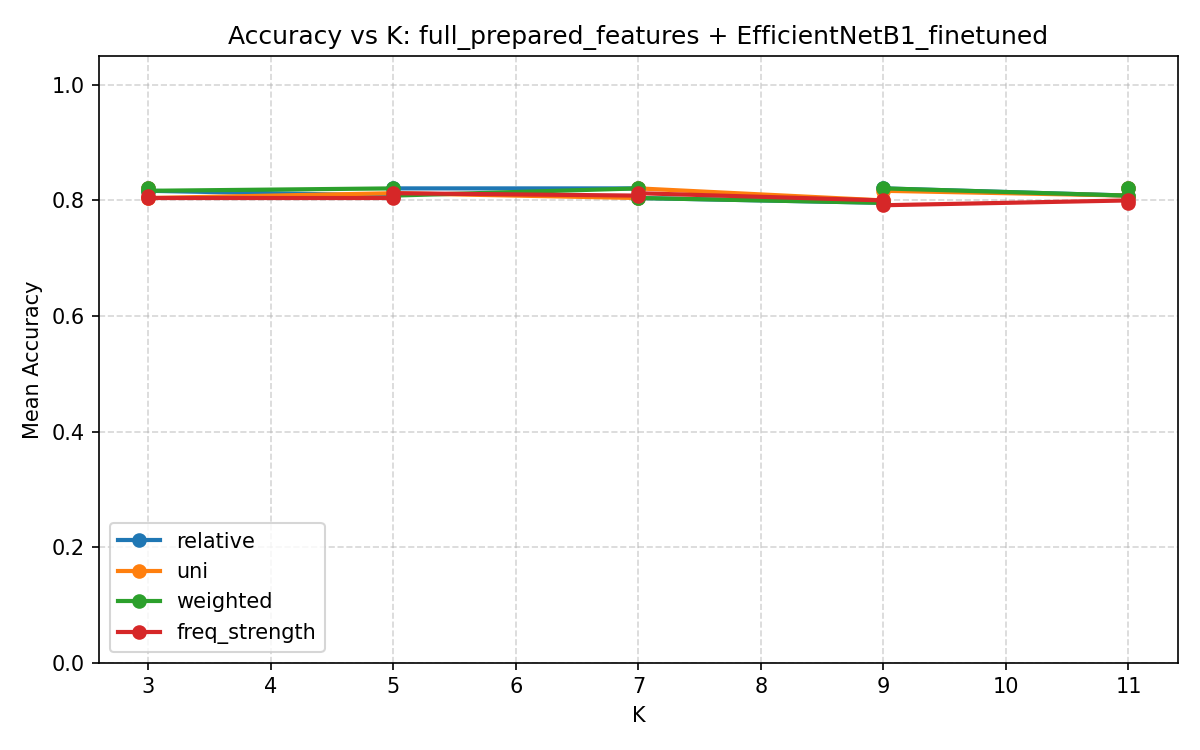
\includegraphics[width=0.49\textwidth,height=0.60\textheight,keepaspectratio]{05_cross_validation/cv_accuracy_vs_k_fullprepared.png}
    \hfill
    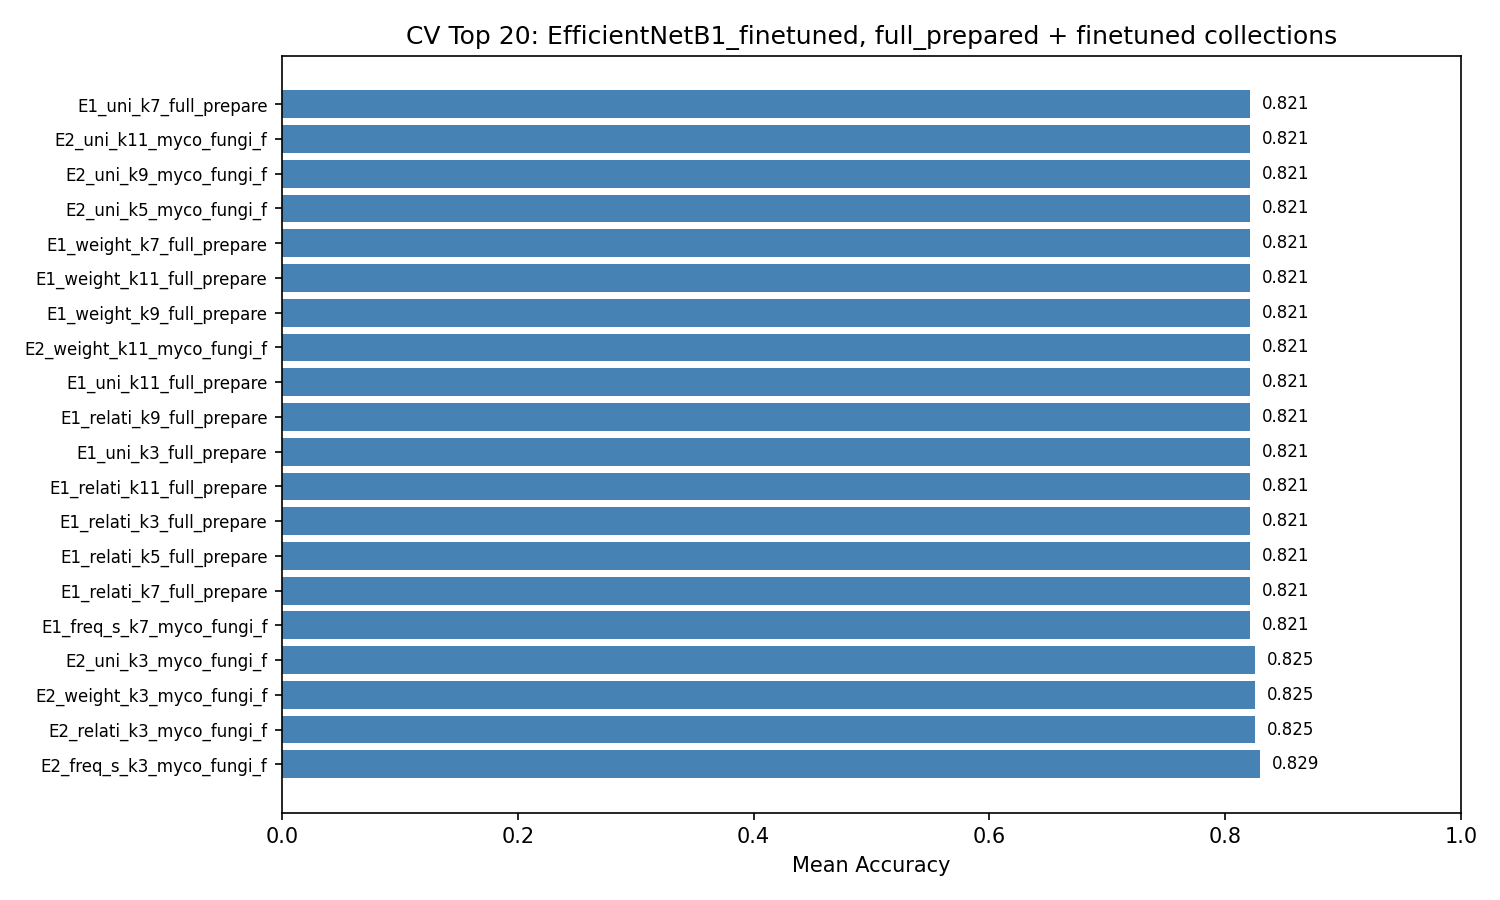
\includegraphics[width=0.49\textwidth,height=0.60\textheight,keepaspectratio]{05_cross_validation/cv_best_configs_new.png}
    \caption{Left: Accuracy vs K (all strategies). Right: Best configurations -- \texttt{EfficientNetB1\_finetuned}. Top CV: \texttt{E2, freq\_strength, k=3} = 0.829}
  \end{figure}
\end{frame}

\begin{frame}{Retrieval: Feature Extractor Comparison}
  \begin{figure}
    \centering
    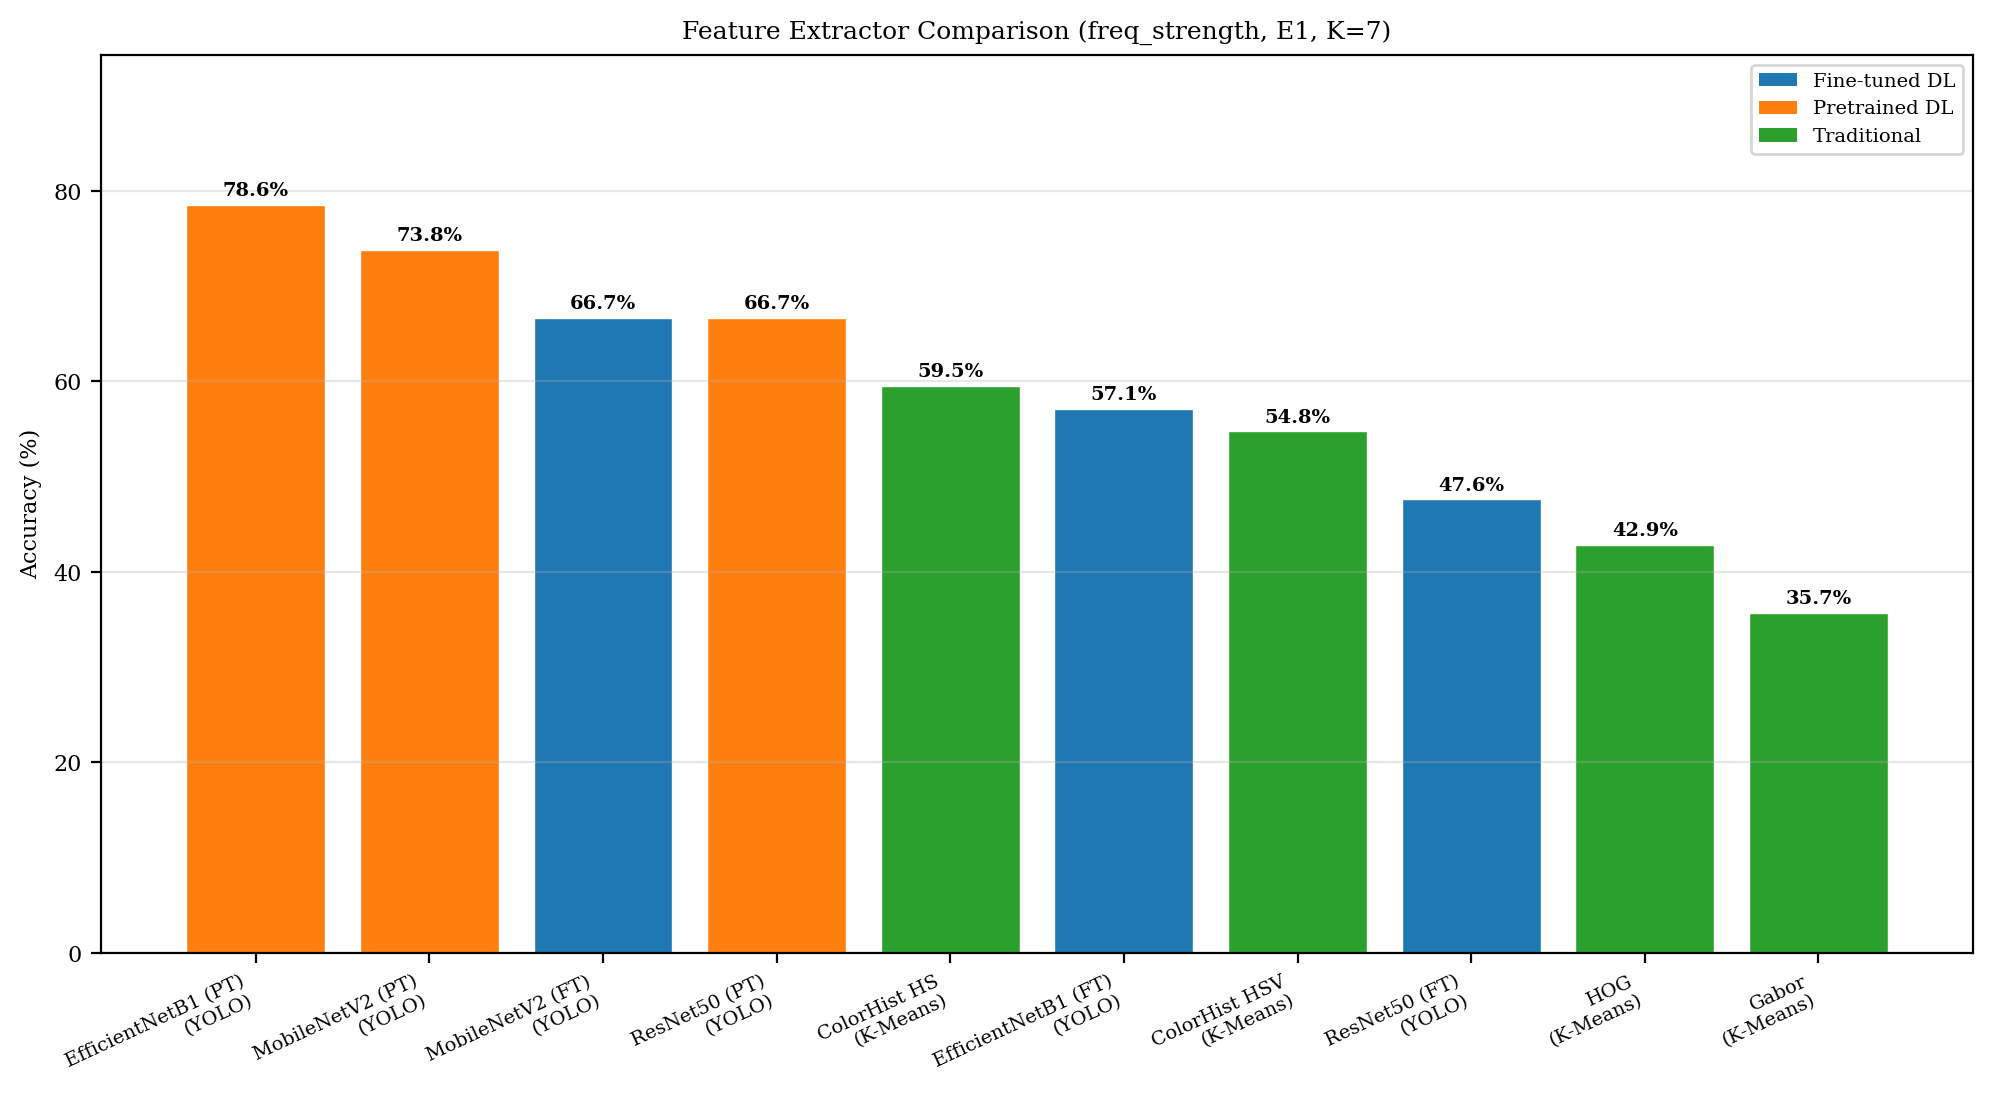
\includegraphics[width=\textwidth,height=0.72\textheight,keepaspectratio]{06_retrieval/extractor_comparison.png}
    \caption{Accuracy by feature extractor family (Fine-tuned = blue, Pretrained = orange, Traditional = green)}
  \end{figure}
\end{frame}

\begin{frame}{Retrieval: Top Configurations}
  \begin{figure}
    \centering
    
\includegraphics[width=\textwidth,height=0.72\textheight,keepaspectratio]{06_retrieval/retrieval_top_configs.png}
    \caption{Top retrieval configurations ranked by accuracy}
  \end{figure}
\end{frame}

\begin{frame}{Retrieval: Staircase Progress}
  \begin{figure}
    \centering
    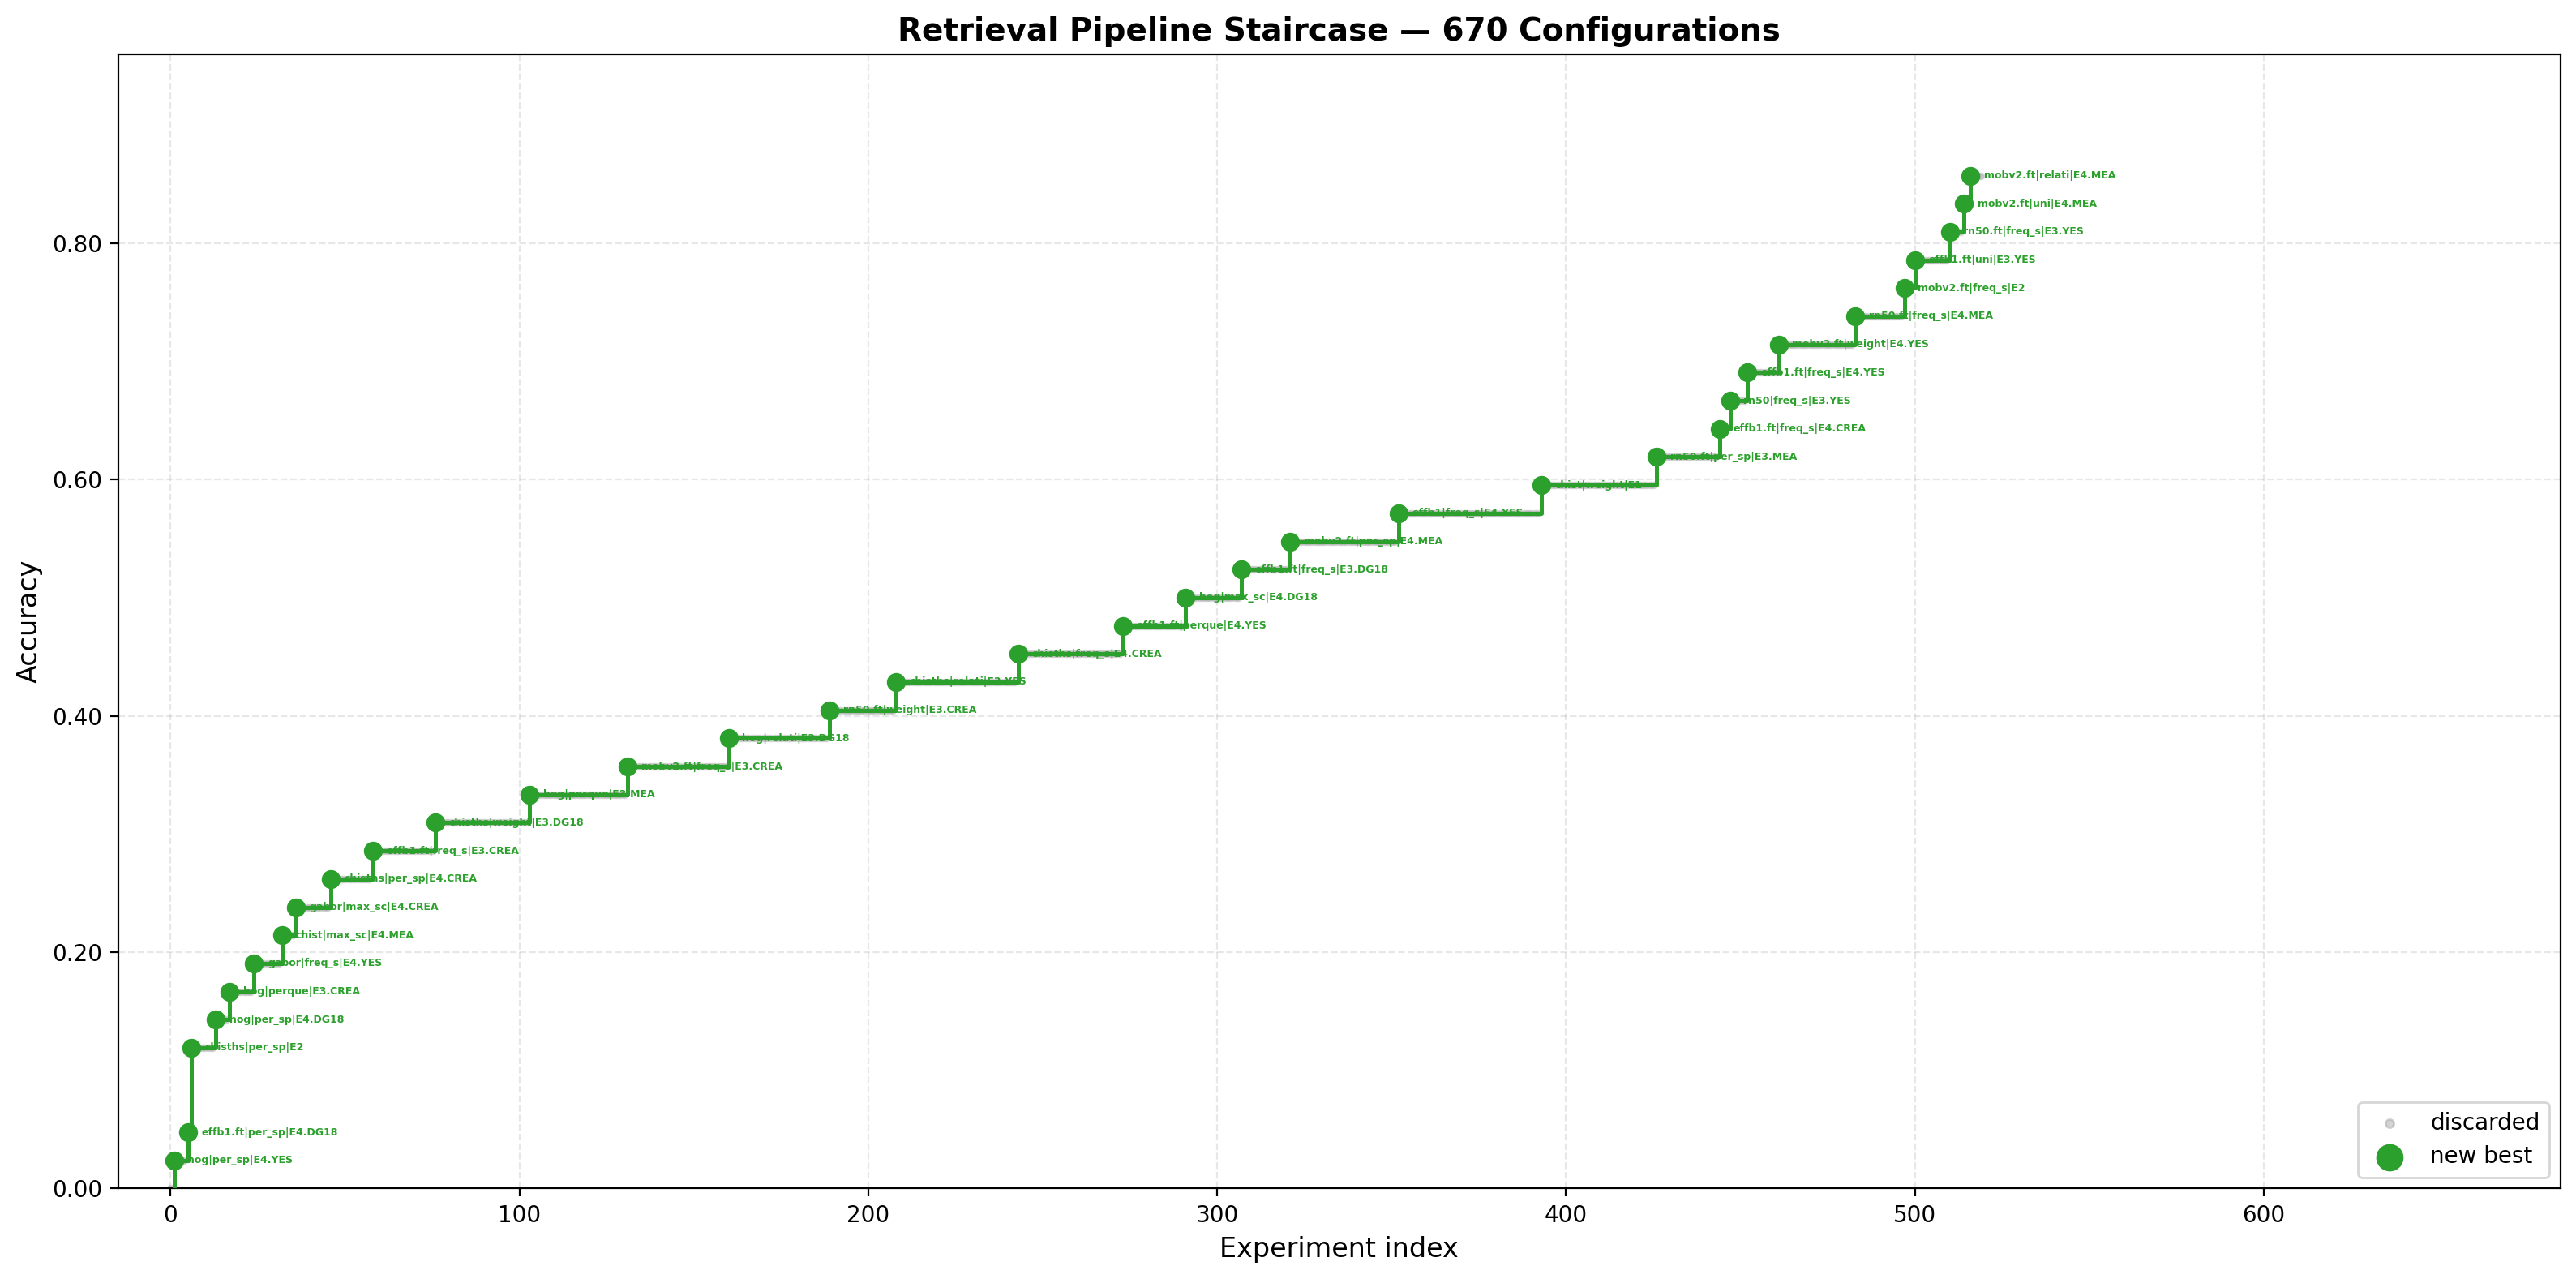
\includegraphics[width=\textwidth,height=0.65\textheight,keepaspectratio]{06_retrieval/staircase_retrieval.png}
    \caption{Experiment staircase: each dot = one experiment, green = new best, gray = below best}
  \end{figure}

  \begin{itemize}
    \item \texttt{weighted} and \texttt{uni} strategies tested across all configs
    \item New \texttt{relative} and \texttt{freq\_strength} strategies added
    \item Ensemble analysis enables combining multiple extractor predictions
  \end{itemize}
\end{frame}

% ======================================================================
\section{Summary}
% ======================================================================

\begin{frame}{Summary \& Key Results}
  \begin{block}{Four Areas of Progress}
    \begin{enumerate}
      \item \textbf{YOLO Segmentation}: Re-run confirmed 0.833 accuracy; equivalent to K-Means but GPU-accelerated
      \item \textbf{Threshold Detection}: 576 experiments; best F1 = 0.407 (\texttt{exp\_decay\_15} + \texttt{f1\_grid})
      \item \textbf{Image Storage}: Robust dual-backend (local + S3) with full API endpoints; tests pass
      \item \textbf{Retrieval Aggregation}: 8 strategies benchmarked; \texttt{weighted} + \texttt{uni} + \texttt{relative} + \texttt{freq\_strength}; best accuracy = 0.833
    \end{enumerate}
  \end{block}

  \begin{center}
    \Large \alert{Thank you!}
  \end{center}
\end{frame}

\end{document}
